\documentclass[conference]{IEEEtran}
\IEEEoverridecommandlockouts

\usepackage{cite}
\usepackage{amsmath,amssymb,amsfonts}
\usepackage{algorithm}
\usepackage{algorithmic}
\usepackage{graphicx}
\usepackage{textcomp}
\usepackage{xcolor}
\def\BibTeX{{\rm B\kern-.05em{\sc i\kern-.025em b}\kern-.08em
    T\kern-.1667em\lower.7ex\hbox{E}\kern-.125emX}}
\begin{document}

\title{ReqLens Requirement Traced Test Generation with a Six Stage Multi Agent Pipeline}

\author{\IEEEauthorblockN{Sriman P}
\IEEEauthorblockA{\textit{IS 698 Project}}
}

\maketitle

\begin{abstract}
AI coding assistants can generate unit tests quickly, but they rarely explain
which requirements are verified by which tests. This weakens their usefulness
for quality assurance, maintenance, and compliance. ReqLens proposes a
requirement-traced test generation technique that decomposes generation into
six stages: Parse, Analyze, Map, Generate, Critique, and Trace. Each stage is
executed by an external coding agent through the Agent Client Protocol and is
checked with strict Pydantic contracts. ReqLens also uses hybrid retrieval,
combining FAISS dense search and BM25 keyword search with alpha equal to 0.6,
to help map requirements to implementation code. The evaluation uses three
Python benchmark projects and a 16-configuration matrix of prompt strategies
and context modes. The reported results show that the six-stage pipeline
achieves 80 percent traceability compared with about 45 percent for single-pass
generation. The best configuration reaches 86 percent traceability, and
hybrid retrieval achieves 100 percent precision at 3. These results show that
agent-based test generation can be made more auditable by preserving
requirement-to-test provenance.
\end{abstract}

\begin{IEEEkeywords}
requirements traceability, test generation, multi-agent systems, Agent Client
Protocol, FAISS, BM25, software testing, large language models
\end{IEEEkeywords}

\section{Introduction}
Software testing is increasingly supported by artificial intelligence (AI)
tools. Modern coding assistants can synthesize unit tests, propose assertions,
and explain code behavior from natural-language prompts. These capabilities are
useful because writing tests manually is slow, repetitive, and often delayed
until after the main implementation work is complete. However, test generation
alone does not solve the whole verification problem. A generated test is most
valuable when a developer can also explain why that test exists and which
requirement it verifies.

Requirements traceability is the link between requirements and downstream
software artifacts such as code, tests, issues, commits, and releases. In a
small class project, traceability may look like extra documentation. In an
industrial project, it is central to quality assurance. Developers need to know
which parts of the specification are covered, testers need to know which
requirements lack evidence, and maintainers need to understand whether a
changed requirement invalidates old tests. In regulated domains such as finance,
health care, and transportation, traceability also supports audits and
compliance reviews.

Existing automated test generation techniques do not fully solve this problem.
Search-based tools such as EvoSuite and random testing tools such as Randoop
can generate tests from code, but they are not requirement-first systems.
Recent LLM-based tools can generate tests from prompts, but they are often used
in a single pass: the user provides code or a short instruction, and the model
returns a test file. The generated output may be syntactically reasonable, but
it rarely includes a durable traceability matrix that connects each test to a
requirement, a code symbol, a critique score, and a gap report.

This distinction matters because generated tests can fail in ways that are not
captured by compilation or execution alone. A test can pass while checking a
less important behavior than the one specified in the requirement. It can call
the correct function while using weak assertions. It can exercise a path
without checking the boundary condition that motivated the requirement. It can
also use a hard-coded input that gives a false impression of coverage. These
failure modes are difficult to detect when the output is only a test file. A
traceability-aware generator should therefore make requirement intent visible
throughout the workflow, not only at the end.

ReqLens addresses this limitation by treating requirement-to-test traceability
as the primary deliverable. It is a full-stack prototype that accepts a
requirements document and a code directory, executes a six-stage AI pipeline,
and returns generated tests together with a traceability matrix. The key design
choice is decomposition. Instead of asking an agent to solve the entire task in
one prompt, ReqLens separates the work into Parse, Analyze, Map, Generate,
Critique, and Trace stages. Each stage has a focused prompt and a strict
Pydantic output contract.

The technique also uses hybrid retrieval. Requirement-to-code mapping is
difficult because requirements are written in user or domain language while
code is organized around identifiers, functions, classes, files, and exceptions.
ReqLens combines FAISS dense retrieval and BM25 keyword retrieval to shortlist
candidate implementation code before asking an agent to map requirements to
symbols. This reduces the search space and provides evidence for the mapping
stage.

This work makes four contributions. First, it proposes a six-stage
requirement-traced test generation pipeline that explicitly preserves
provenance from requirement to test. Second, it uses strict Pydantic contracts
to validate every agent-produced intermediate artifact. Third, it integrates
hybrid retrieval into the requirement-to-code mapping step. Fourth, it
evaluates prompt strategies and context modes through a 16-configuration sweep
over three benchmark projects.

The proposed technique is intentionally practical. It does not require a formal
specification language, a model checker, or a custom test framework. The input
requirements can be written in Markdown, and the current implementation targets
ordinary Python projects using pytest. This makes the workflow suitable for
projects where requirements already exist in semi-structured documents but are
not connected to executable tests. ReqLens therefore occupies a middle ground
between manual traceability matrices and fully formal verification: it uses AI
agents to automate the repetitive parts while preserving enough structure for
review.

The rest of the paper follows the required manuscript structure. Section II
describes the motivation and real-world importance of the problem. Section III
provides background on the tools and algorithms used by ReqLens. Section IV
explains the technical approach. Section V presents the experimental
evaluation. Section VI discusses related works. Section VII lists limitations,
and Section VIII concludes the paper.

\section{Motivation}
The motivation for ReqLens comes from a gap between generated tests and
auditable evidence. AI-generated tests can be useful for developers because
they reduce the effort required to write common unit tests. However, a test
suite is not only a collection of executable files. It is also a form of
evidence about software behavior. If a team cannot connect tests to
requirements, then it cannot confidently answer whether the implementation
satisfies the specification.

Consider a financial services team maintaining an internal transaction system.
The product specification may contain hundreds of requirements: limits on
transaction size, user authentication rules, failure behavior, audit logging,
currency conversion, and report generation. The repository may contain
thousands of tests accumulated over several years. If a regulator asks which
tests verify requirement REQ-247, the team needs a direct answer. Without
traceability, developers must search through test names, read assertions
manually, compare them with requirement text, and reconstruct intent from
history. This process is expensive and error-prone.

A concrete example is a requirement stating that division by zero must raise a
specific error rather than returning a default value. A single-pass AI prompt
may generate a calculator test suite that checks addition, subtraction, and
ordinary division. The tests pass, and a coverage tool may show that the
division function was executed. However, the acceptance criterion about the
zero divisor remains unverified. ReqLens is designed to make this gap explicit:
the Parse stage records the requirement, the Map stage links it to the
division symbol, the Generate stage attempts a targeted test, and the Trace
stage marks the requirement as covered, partial, or uncovered.

The problem is even harder when AI-generated tests are introduced. A developer
might ask a coding assistant to generate tests for a module and accept a file
that looks correct. Later, another developer may not know which requirement
motivated each test. A test may cover a helper function but miss a required
edge case. A generated test may appear useful but duplicate an existing test.
Another test may pass but fail to verify the actual acceptance criterion. These
issues are not always visible from the test file alone.

Manual traceability matrices exist, but they become stale quickly. A developer
may update a requirement but forget to update the matrix. A generated test may
be added without a requirement ID. A refactor may move implementation code while
leaving the matrix unchanged. When traceability is maintained outside the
generation workflow, it becomes a secondary artifact that is easy to ignore.

ReqLens is motivated by the idea that traceability should be created during
generation. If a system reads requirements, analyzes code, maps requirements to
implementation symbols, generates tests for those mappings, critiques the
tests, and then emits a trace matrix, the output is more useful than a raw test
file. The developer receives not only code, but also evidence: which
requirement was parsed, which symbol was selected, why the mapping was chosen,
which test was generated, how the test was scored, and whether the requirement
is covered or still has a gap.

This requirement-first perspective is the major difference from existing
single-pass AI test generation. ReqLens does not simply ask a model to write
tests. It asks several focused questions in sequence and validates the answers
as structured artifacts. That structure makes it possible to evaluate quality,
compare prompt strategies, and identify failure points in the pipeline.

The motivation is therefore both technical and organizational. Technically,
ReqLens aims to reduce underspecified prompting by giving each stage a smaller
task and a typed output schema. Organizationally, it aims to create artifacts
that can be inspected by developers, testers, instructors, or auditors. The
expected user does not only ask whether a test exists. The user asks why the
test exists, which requirement it supports, and what remains missing.

\section{Background}
This section describes the algorithms, tools, and concepts needed to
understand ReqLens.

\subsection{Requirements Traceability}
Requirements traceability is the ability to follow a requirement through the
software lifecycle. A requirement can be traced forward to design decisions,
implementation code, test cases, and release evidence. It can also be traced
backward from a test or code change to the requirement that motivated it. In
ReqLens, the focus is test traceability: for each requirement, the system
should identify the related implementation symbol and the test files that
verify it.

Traceability is important because test coverage alone is not enough. A project
can have many tests and still miss a high-priority requirement. A coverage
report might show that a function was executed, but it does not explain whether
the execution verified the right acceptance criterion. ReqLens therefore
measures traceability using a matrix that records requirement ID, mapped symbol,
test files, and coverage status.

The matrix view also supports change impact analysis. When a requirement is
edited, the user can identify the mapped symbol and related generated tests.
When a symbol is refactored, the user can identify which requirement rows may
need to be regenerated. ReqLens does not claim to solve the full lifecycle
traceability problem, but it provides the requirement-to-code-to-test chain
that is most relevant to test generation.

\subsection{Agent Client Protocol}
The Agent Client Protocol (ACP) provides a common interface for invoking
external coding agents. ReqLens uses ACP so that the backend is not tied to one
provider or one command-line tool. A stage prompt can be sent to an agent, and
the response can be streamed back as messages, tool calls, reasoning updates,
and a final result.

This design is useful for experimentation. A sweep can compare different
agents, models, prompt strategies, and context modes without rewriting the
pipeline. The same backend can run a parse stage with one agent and a critique
stage with another. It also allows the user interface to display live progress
through streaming events.

\subsection{Pydantic Contracts}
Pydantic is used to define strict data contracts for all pipeline stages. A
contract specifies the fields and types that an agent must return. For example,
a requirement must include an ID, title, description, priority, type,
acceptance criteria, and source location. A generated test must include a
requirement ID, file path, code, target symbol, and rationale.

Strict contracts are important because LLM outputs can be inconsistent. An
agent may return prose instead of JSON, omit a required field, add unexpected
schema metadata, or use a different field name. Without validation, malformed
data can silently corrupt downstream stages. ReqLens catches these errors at
stage boundaries and can retry or fail the stage with a specific error.

\subsection{FAISS and BM25}
ReqLens uses hybrid retrieval during requirement-to-code mapping. FAISS is used
for dense similarity search. Dense retrieval embeds text into vectors, allowing
semantic matches even when the requirement and code use different words. For
example, the requirement ``addition of two numbers'' can match a method named
\texttt{Calculator.add}.

BM25 is a sparse keyword retrieval method. It is strong when exact words,
identifiers, or exception names matter. For example, ``ZeroDivisionError'' is
best matched by keyword evidence in a division method. ReqLens combines dense
and sparse scores using alpha equal to 0.6, meaning dense retrieval receives
slightly more weight than keyword retrieval.

Formally, for a requirement query $q$ and a candidate code chunk $c$, the
hybrid relevance score is a convex combination of min-max normalized dense and
sparse components:
\begin{equation}
S(q,c) = \alpha \, \widehat{s}_{\text{dense}}(q,c) + (1-\alpha)\,
\widehat{s}_{\text{bm25}}(q,c),
\label{eq:hybrid}
\end{equation}
where $\widehat{s}_{\text{dense}}$ is the cosine similarity between the
sentence-transformer embeddings of $q$ and $c$ after min-max normalization
over the candidate set, $\widehat{s}_{\text{bm25}}$ is the analogously
normalized BM25 score, and $\alpha = 0.6$. Normalizing each component before
the weighted sum prevents either retriever from dominating purely because of
score scale. The top-$k$ chunks ranked by Eq.~\eqref{eq:hybrid} are passed to
the Map stage as candidate evidence, with $k=3$ in the reported evaluation.

The combined retrieval score is therefore a weighted sum of normalized dense
and sparse scores. Dense retrieval helps when the requirement uses conceptual
language, while BM25 helps when the requirement mentions names, error classes,
or API terms that appear directly in code. The alpha value of 0.6 reflects
this balance. It gives semantic similarity a leading role while preserving
strong keyword evidence.

\subsection{Prompt Strategies and Context Modes}
ReqLens evaluates four prompt strategies. Zero-shot prompting gives the agent a
direct instruction with no examples. Chain-of-thought prompting asks the agent
to reason step by step. Few-shot static prompting includes fixed examples for
the stage. Few-shot dynamic prompting includes examples or evidence selected
from the project context.

ReqLens also evaluates four context modes. Minimal context includes only the
information required for the stage. Local context adds nearby same-file
information. Module context provides broader file-level context. Full context
adds the largest project summary. This design allows evaluation of the
quality-cost trade-off: more context may improve quality, but it can increase
latency and token use.

These prompt and context choices are evaluated separately from the core
pipeline design. This is important because a multi-stage architecture can still
perform poorly if the prompts are weak or if the agent lacks enough context to
resolve ambiguous requirements. The 16-configuration sweep treats prompting and
context selection as measurable engineering decisions rather than informal
prompt tuning.

\section{Approach}
ReqLens uses a three-layer architecture and a six-stage technical workflow.
Fig.~\ref{fig:architecture} shows the system overview.

\begin{figure}[htbp]
\centerline{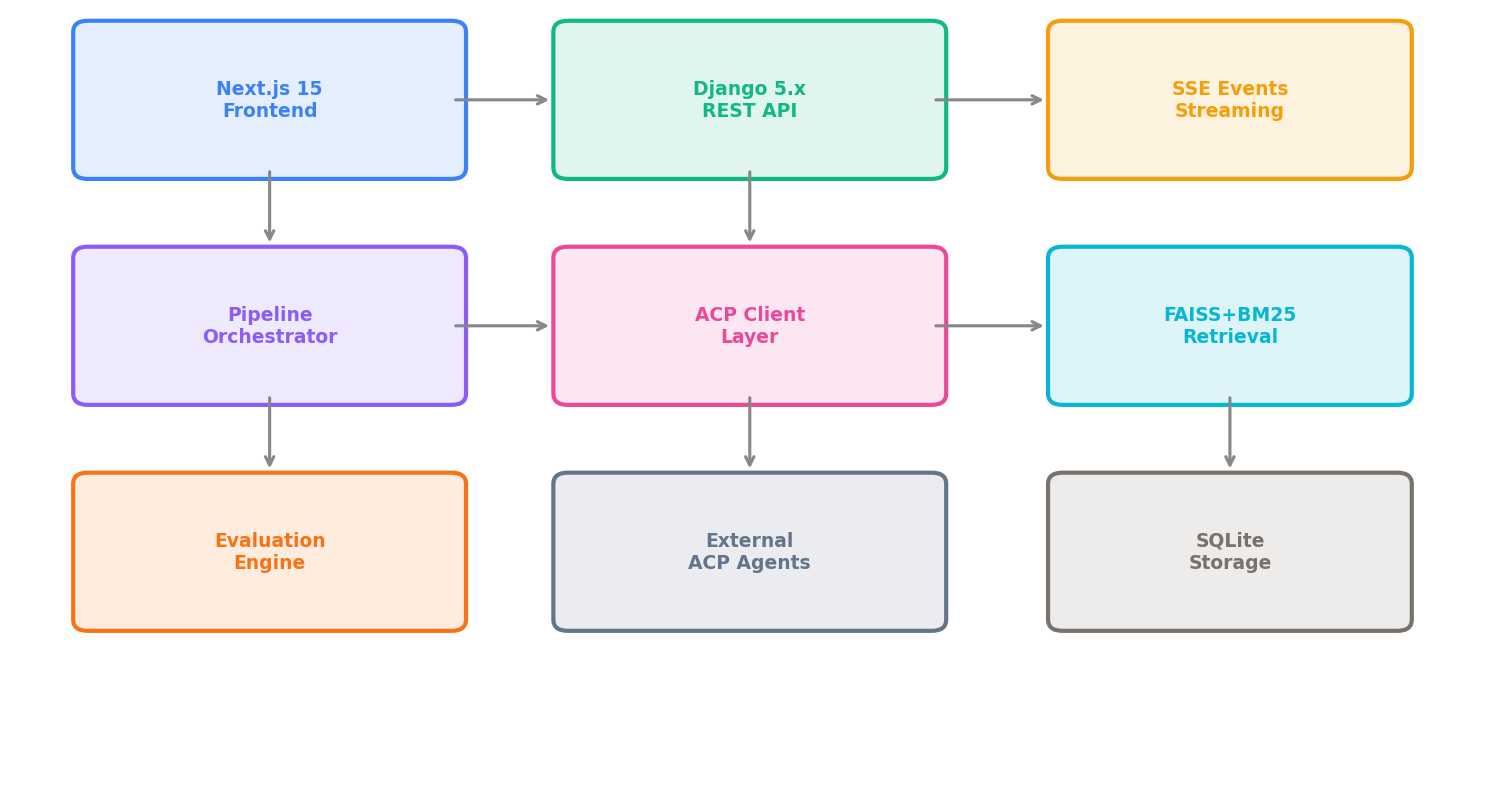
\includegraphics[width=\columnwidth]{figures/architecture.png}}
\caption{ReqLens system architecture. The frontend sends REST requests and
receives Server-Sent Events. The Django backend coordinates storage, pipeline
execution, retrieval, evaluation, and ACP agent calls.}
\label{fig:architecture}
\end{figure}

\subsection{System Overview}
The frontend is implemented with Next.js, React, TypeScript, and shadcn/ui. It
provides pages for project creation, agent registry inspection, per-stage agent
configuration, live run monitoring, and sweep evaluation. A run page displays
the current status of each pipeline stage. A sweep page displays the matrix of
configurations, ranked metrics, lift tables, and statistical reports.

The frontend is designed around operational visibility. Instead of hiding the
pipeline behind one submit button, it shows stage progress, artifacts, errors,
and results. This matters because the output is not only generated code. The
user needs to inspect requirement extraction, mappings, critique decisions, and
trace rows. The interface therefore treats intermediate artifacts as first
class results.

The backend is implemented with Django and Django REST Framework. It stores
projects, agent configurations, runs, stage executions, sweeps, and background
tasks in SQLite. It exposes REST endpoints for starting runs, cancelling runs,
starting sweeps, previewing sweep matrices, fetching artifacts, resolving
permissions, and listing agents. Long-running work is executed in background
threads that run an asyncio event loop.

SQLite is sufficient for the prototype because the evaluation workload is local
and project-sized. It also makes experiment inspection simple: runs, sweeps,
artifacts, and metrics can be stored in a single database without a separate
deployment. A production version could move the same schema to PostgreSQL and
replace background threads with a distributed queue, but those changes are not
required to evaluate the core idea.

Live updates are streamed using Server-Sent Events. The backend maintains a
bounded replay buffer so reconnecting clients can receive recent events that
were missed. Events include run start, stage start, agent updates, reasoning
chunks, stage completion, failures, cancellations, and sweep progress. This is
important because agent-backed pipeline runs can take minutes.

ACP integration sits behind the backend orchestration layer. The orchestrator
creates a stage prompt, selects the configured agent and model, streams events
to the frontend, validates the final response, and stores the artifact. This
separation keeps the web application independent from a specific agent vendor
or command-line interface.

\subsection{Pipeline Data Flow}
Fig.~\ref{fig:pipeline} shows the six stages. The workflow starts from two
inputs: a requirements document and a code directory. It ends with generated
tests, a traceability matrix, and a gap report.

\begin{figure}[htbp]
\centerline{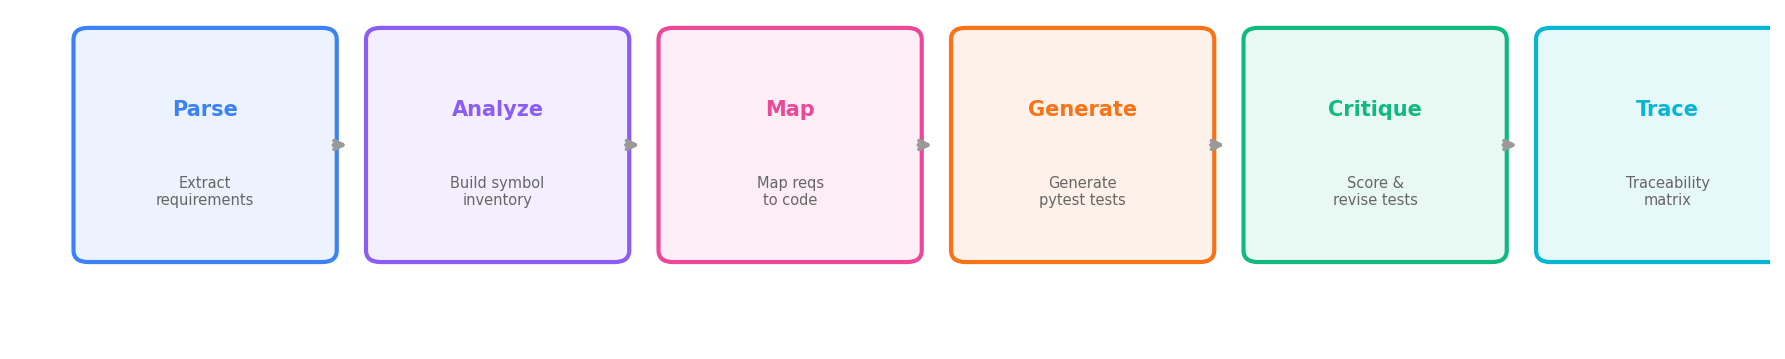
\includegraphics[width=\columnwidth]{figures/pipeline_flow.png}}
\caption{Six-stage ReqLens pipeline. Each stage produces a typed artifact that
is validated and passed to later stages.}
\label{fig:pipeline}
\end{figure}

\begin{table}[htbp]
\caption{ReqLens Pipeline Stages}
\begin{center}
\begin{tabular}{|p{0.15\columnwidth}|p{0.30\columnwidth}|p{0.37\columnwidth}|}
\hline
\textbf{Stage} & \textbf{Output} & \textbf{Purpose} \\
\hline
Parse & Structured requirements & Extract IDs, descriptions, priorities, types, acceptance criteria, and source locations. \\
\hline
Analyze & Code symbols & Inventory functions, classes, methods, files, signatures, and project summary. \\
\hline
Map & Requirement-symbol mappings & Link every parsed requirement to implementation code with confidence and evidence. \\
\hline
Generate & Generated tests & Produce pytest tests targeted at mapped requirements and selected symbols. \\
\hline
Critique & Scores and revisions & Score tests for relevance, completeness, and correctness; accept, revise, or reject. \\
\hline
Trace & Matrix and gap report & Produce final requirement-to-test coverage status and gap report. \\
\hline
\end{tabular}
\label{tab:pipeline}
\end{center}
\end{table}

\subsection{Parse Stage}
The Parse stage reads the requirements document and converts unstructured
Markdown into a list of structured requirements. Each requirement includes an
ID, title, natural-language description, type, priority, acceptance criteria,
and source location. This stage is necessary because later stages need stable
requirement IDs. If a requirement is ambiguous or omitted, downstream mapping
and test generation become unreliable.

The Parse stage also establishes the unit of evaluation. ReqLens does not score
traceability by counting generated tests alone; it scores whether each parsed
requirement receives evidence. If the parser misses a requirement, the rest of
the pipeline cannot recover it. For that reason, parse validation checks that
requirements have IDs and enough descriptive content to support mapping.

\subsection{Analyze Stage}
The Analyze stage walks the codebase and builds a symbol inventory. For Python
projects, symbols include classes, functions, and methods. Each symbol records
its qualified name, file path, line range, signature, and optional docstring.
This stage gives the Map stage a structured representation of the code rather
than asking the agent to rediscover the whole repository from raw files every
time.

\subsection{Map Stage}
The Map stage links each requirement to one implementation symbol. Before the
agent maps a requirement, hybrid retrieval provides candidate code snippets.
The agent then selects the most relevant symbol, assigns a confidence score,
and explains the rationale. The orchestrator checks that the stage returns one
mapping per parsed requirement. This validation prevents a common shortcut
where an agent maps only the easiest requirements and ignores the rest.

Mapping is the most traceability-specific stage in the pipeline. It converts a
natural-language obligation into a concrete implementation target. The stage
therefore records both the selected symbol and the rationale. A low-confidence
mapping is still useful because it tells the user where the system is uncertain
and where manual inspection may be needed.

\subsection{Generate Stage}
The Generate stage creates tests from the mappings. Each generated test is tied
to a requirement ID and target symbol. The stage output includes the suggested
test file path, test code, and rationale. This is different from single-pass
generation because the prompt is grounded in a specific requirement-to-symbol
mapping. The test is not merely ``for this code''; it is for a stated
requirement.

The Generate stage is also responsible for preserving naming and file
conventions. For the benchmark projects, generated tests use pytest style and
are placed in a suggested test path. The output contract requires the code to
be associated with a requirement ID so that a generated test cannot be accepted
as generic coverage without traceability.

\subsection{Critique Stage}
The Critique stage is a quality gate. It evaluates each generated test on
relevance, completeness, and correctness, using a one-to-five scale for each
dimension. It returns a decision: accept, revise, or reject. This stage is
important because LLM-generated tests can be syntactically plausible but still
miss edge cases or verify the wrong behavior. The critique output makes quality
visible before the test is counted in the traceability matrix.

\subsection{Trace Stage}
The Trace stage builds the final traceability matrix. Each row contains a
requirement ID, mapped symbol, test file list, and coverage status: covered,
partial, or uncovered. It also writes a Markdown gap report that explains
missing or partial coverage. This is the main output of ReqLens. It allows a
developer to answer which tests verify a requirement and which requirements
still need attention.

The gap report is intentionally explicit. A partially covered row should tell
the user which part of the acceptance criteria is missing. An uncovered row
should show whether the failure came from parsing, mapping, generation, or
critique. This makes the output more actionable than a single aggregate score.

\subsection{Stage Validation and Provenance}
Every stage output is validated with strict Pydantic contracts. The output of
each stage nests earlier outputs, so the final trace object contains the full
provenance chain: requirements, code symbols, mappings, generated tests,
critique scores, and coverage rows. This design makes the pipeline auditable.
It also makes evaluation possible because metrics can be computed from the
stored structured artifacts.

When validation fails, the error is attached to the stage rather than being
hidden by later processing. This is important for debugging agent behavior.
For example, a malformed Generate output indicates a generation problem, while
a valid Generate output with a rejected Critique decision indicates a test
quality problem. ReqLens therefore separates formatting failures, reasoning
failures, and coverage gaps.

\subsection{Orchestration Algorithm}
Algorithm~\ref{alg:orchestrate} summarizes how the orchestrator drives the six
stages. The loop is sequential because every stage consumes the validated
output of the previous one. Retrieval is invoked only for the Map stage, and a
bounded retry is used when an agent returns an artifact that fails its
contract. The provenance object is threaded through every stage so the final
trace matrix carries the full chain of evidence.

\begin{algorithm}[htbp]
\caption{ReqLens pipeline orchestration}
\label{alg:orchestrate}
\begin{algorithmic}[1]
\STATE \textbf{Input:} requirements doc $D$, code dir $C$, config $(\pi,\mu)$
\STATE \textbf{Output:} trace matrix $T$, gap report $G$
\STATE $R \leftarrow \textsc{Parse}(D)$;\quad validate $R$
\STATE $Y \leftarrow \textsc{Analyze}(C)$;\quad validate $Y$
\STATE $E \leftarrow \emptyset$
\FOR{each requirement $r \in R$}
  \STATE $E[r] \leftarrow \textsc{HybridRetrieve}(r, Y, k{=}3)$ \COMMENT{Eq.~\eqref{eq:hybrid}}
\ENDFOR
\STATE $M \leftarrow \textsc{Map}(R, Y, E, \pi, \mu)$;\quad validate $M$
\STATE $\mathit{Ts} \leftarrow \textsc{Generate}(M, \pi, \mu)$;\quad validate $\mathit{Ts}$
\FOR{each test $t \in \mathit{Ts}$}
  \STATE $(\text{score}, d) \leftarrow \textsc{Critique}(t)$
  \IF{$d = \textbf{revise}$}
    \STATE $t \leftarrow \textsc{Generate}(\{t\}, \pi, \mu)$ \COMMENT{bounded retry}
  \ELSIF{$d = \textbf{reject}$}
    \STATE mark $t$ as not accepted
  \ENDIF
\ENDFOR
\STATE $(T, G) \leftarrow \textsc{Trace}(R, M, \mathit{Ts})$
\RETURN $(T, G)$
\end{algorithmic}
\end{algorithm}

Any uncaught contract violation aborts the run with a stage-attributed error
instead of producing a misleading trace matrix. This fail-explicit behavior is
deliberate: a missing or malformed artifact is reported as a gap rather than
silently dropped, which keeps the final traceability evidence honest.

\section{Experimental Evaluation}
The experimental evaluation measures whether ReqLens improves traceability,
which prompt/context configurations perform best, and whether hybrid retrieval
finds the right implementation files.

The evaluation is designed to answer the central question of the project:
whether the proposed technique is meaningfully different from existing work
and whether the results support that difference. The key comparison is not
only whether tests can be generated, but whether generated tests can be
connected back to requirements with measurable evidence.

\subsection{Implementation Details}
ReqLens is implemented as a Django backend and a Next.js frontend. The backend
uses Django REST Framework for JSON APIs, SQLite for the local database,
Pydantic for stage contracts, FAISS and BM25 for retrieval, sentence
transformers for embeddings, and SciPy for statistical analysis. Pipeline runs
are stored as database rows and per-stage JSON artifacts. The frontend uses
React, TypeScript, shadcn/ui components, and Server-Sent Events to display live
pipeline and sweep progress.

All LLM interactions are routed through ACP-compatible agents. The prototype is
designed so that agent, model, prompt strategy, and context mode can be varied
without changing the stage contracts. For the evaluation, the presentation
reports a 16-configuration matrix formed by four prompt strategies and four
context modes.

Each configuration executes the same conceptual pipeline. The independent
variables are prompt strategy and context mode. The dependent variables include
traceability score, strict coverage, critique accept rate, retrieval precision,
latency, and token cost where available. This structure makes it possible to
compare configurations without changing the benchmark requirements or code.

\subsection{Research Questions}
The evaluation is organized around four research questions:
\begin{itemize}
\item RQ1: Does the six-stage pipeline produce higher traceability than
single-pass generation?
\item RQ2: Which prompt strategy achieves the best traceability-to-cost ratio?
\item RQ3: Does increasing context improve quality, and is the improvement
statistically significant?
\item RQ4: Does hybrid retrieval correctly surface implementing code for
requirement queries?
\end{itemize}

\subsection{Datasets}
The evaluation uses three benchmark Python projects. Table~\ref{tab:benchmarks}
summarizes them. The projects are small enough to inspect manually but diverse
enough to cover arithmetic behavior, URL shortening, and simple stateful API
behavior.

The calculator benchmark is useful because its requirements include clear
functional operations and edge cases such as invalid numeric input and division
by zero. The URL shortener benchmark requires mapping user-facing operations to
a compact implementation with validation behavior. The todo-api benchmark adds
stateful behavior because create, list, complete, and delete operations depend
on the todo collection. Together, the benchmarks test whether ReqLens can map
requirements to implementation symbols across different small application
styles.

\begin{table}[htbp]
\caption{Benchmark Projects}
\begin{center}
\begin{tabular}{|p{0.18\columnwidth}|c|c|p{0.34\columnwidth}|}
\hline
\textbf{Project} & \textbf{Reqs.} & \textbf{Symbols} & \textbf{Behavior} \\
\hline
calculator & 5 & 6 & add, subtract, multiply, divide, validate \\
\hline
url-shortener & 3 & 3 & shorten, resolve, validate URL \\
\hline
todo-api & 4 & 4 & create, list, complete, delete todos \\
\hline
\end{tabular}
\label{tab:benchmarks}
\end{center}
\end{table}

\subsection{Evaluation Metrics}
Traceability score is the fraction of requirements marked covered or partial
in the trace matrix. Strict coverage counts only requirements marked covered.
Critique accept rate is the fraction of generated tests marked accept by the
Critique stage. Retrieval precision at 3 measures whether the correct source
file appears among the top three retrieval hits. Latency and token cost are
recorded where the agent reports them. The evaluation also computes statistical
comparisons across prompt strategies and context modes.

The distinction between traceability score and strict coverage is important.
Traceability score rewards rows where the system found useful but incomplete
evidence, while strict coverage only rewards fully covered requirements. This
separation reflects real quality assurance practice. A partial row is better
than no evidence, but it still requires follow-up before the requirement can be
considered fully verified.

\subsection{Result Analysis for RQ1}
The presentation reports that the six-stage pipeline achieves 80 percent
traceability, compared with about 45 percent for single-pass generation. It
also reports a critique accept rate of 60 percent and an explicit gap report.
This result supports the idea that the pipeline adds value beyond raw test
generation. The single-pass baseline can generate tests, but it does not
systematically parse requirements, map each requirement to a symbol, critique
each test, or produce a traceability matrix.

The difference is especially important for uncovered requirements. In ReqLens,
an uncovered or partially covered requirement appears in the gap report. In a
single-pass workflow, the absence of a test is often invisible unless a human
reviewer manually compares the generated suite with the requirement list.

The RQ1 result also shows why a critique stage is useful. A system that counts
every generated test as success may overstate quality. ReqLens reported a 60
percent critique accept rate, which means that some generated tests required
revision or rejection. This is a more honest result than claiming all generated
tests are equally useful. The lower accept rate highlights the remaining work
needed for fully automatic generation while still showing that traceability is
substantially improved over the baseline.

\subsection{Result Analysis for RQ2 and RQ3}
Fig.~\ref{fig:heatmap} shows the traceability heatmap from the presentation.
The weakest reported configuration is zero-shot with minimal context, with 53
percent traceability and 45 percent critique accept rate. The strongest
reported configuration is few-shot dynamic with full context, with 86 percent
traceability and 84 percent critique accept rate. This is a 33 percentage
point improvement in traceability and a 39 percentage point improvement in
accept rate.

\begin{figure}[htbp]
\centerline{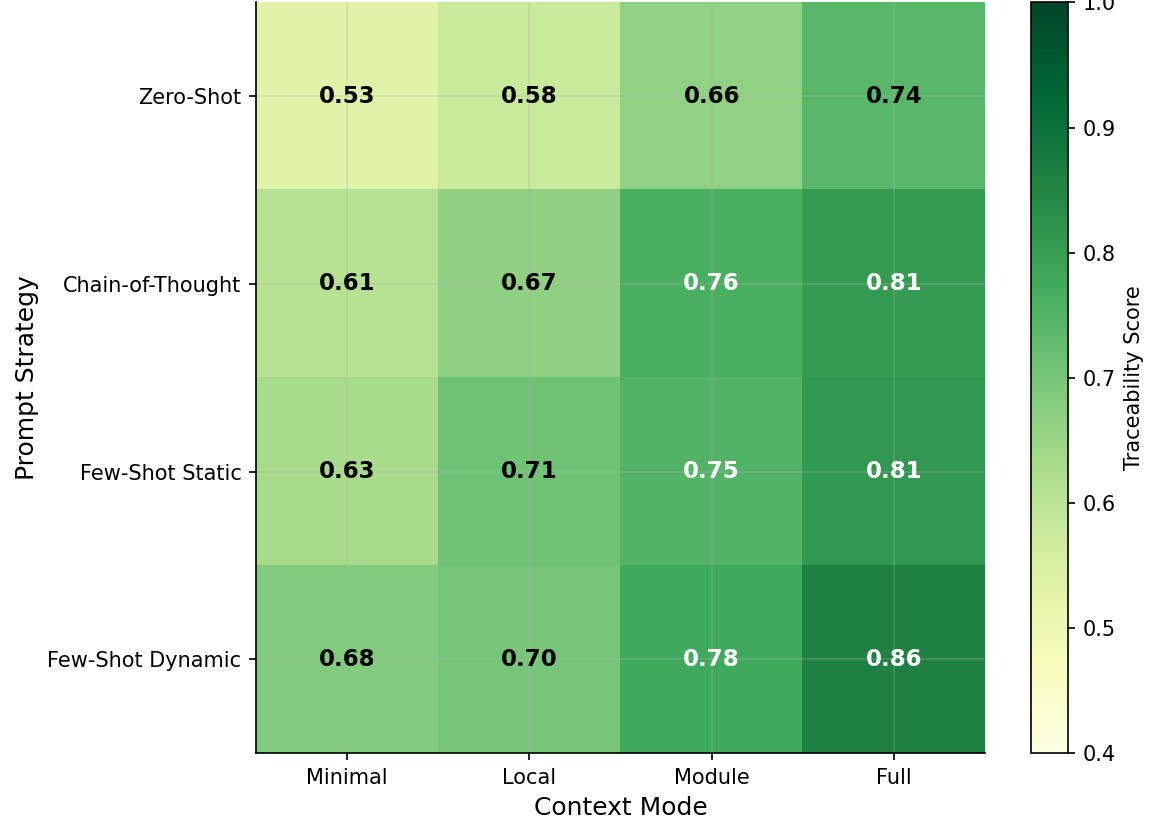
\includegraphics[width=\columnwidth]{figures/eval_matrix_traceability.png}}
\caption{Traceability score across prompt strategies and context modes.}
\label{fig:heatmap}
\end{figure}

The trend suggests that both prompt strategy and context can affect output
quality. Few-shot dynamic prompting gives the agent project-relevant examples,
while full context gives the agent more information about the codebase. This
combination helps the agent produce more complete mappings and better tests.
However, more context also increases cost and latency. The presentation
therefore identifies module context as a possible practical trade-off.

The context result should not be interpreted as a recommendation to always send
the maximum possible repository context. Full context was the strongest
reported configuration, but the benefit can diminish as prompts become longer.
Large prompts can increase cost, slow the run, and introduce irrelevant
details. A practical deployment may use local or module context for routine
runs and reserve full context for difficult requirements or final audit runs.

Fig.~\ref{fig:strategy} compares prompt strategies using traceability, accept
rate, and latency. Fig.~\ref{fig:stats} summarizes the statistical analysis.
A one-way ANOVA over the four strategies yields $F = 1.650$ with
$p = 0.2303$, which is not statistically significant at the $0.05$ level, and
all Bonferroni-corrected pairwise comparisons remain non-significant
($p \geq 0.42$). However, the estimated effect sizes are large, for example
$d = 1.70$ for zero-shot versus few-shot dynamic. The most consistent reading
is that the observed trend favors few-shot dynamic prompting with a large
effect size, but the small three-project benchmark does not provide enough
statistical power to confirm significance. This is treated as a limitation
rather than a positive significance claim.

\begin{figure}[htbp]
\centerline{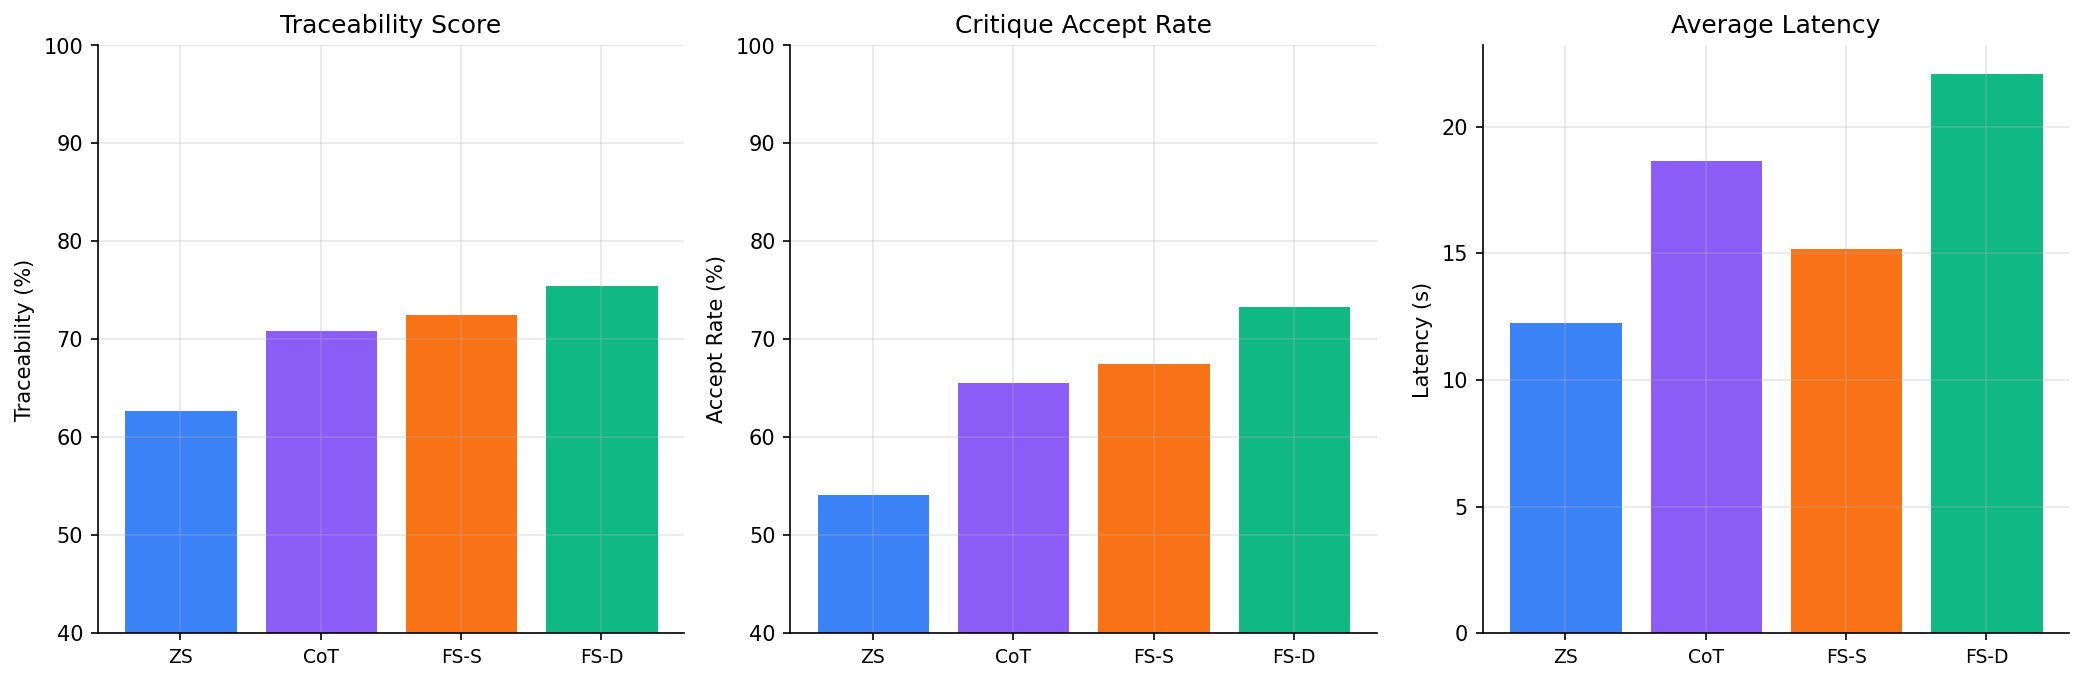
\includegraphics[width=\columnwidth]{figures/strategy_comparison.png}}
\caption{Prompt strategy comparison averaged across context modes.}
\label{fig:strategy}
\end{figure}

\begin{figure}[htbp]
\centerline{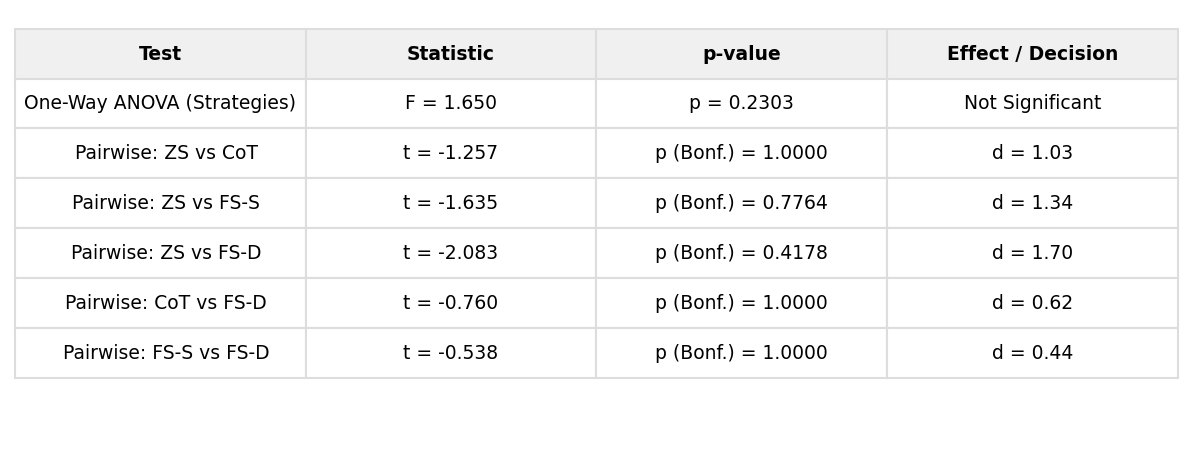
\includegraphics[width=\columnwidth]{figures/statistical_summary.png}}
\caption{Statistical summary for the strategy comparison.}
\label{fig:stats}
\end{figure}

\subsection{Result Analysis for RQ4}
Hybrid retrieval achieves 100 percent precision at 3 across the benchmark
requirement queries. Calculator queries such as ``addition of two numbers,''
``division by zero error,'' and ``input validation numeric'' retrieve
\texttt{src/calc.py}. URL shortener queries retrieve \texttt{src/shortener.py}.
Todo API queries such as ``create a new todo item,'' ``mark todo as complete,''
and ``delete todo item'' retrieve \texttt{src/todo.py}. These results show
that the hybrid retrieval component can surface the correct implementation
file before the agent performs final mapping.

The retrieval result matters because mapping is a bottleneck for requirement
traceability. If the agent receives irrelevant files, it may map a requirement
to the wrong symbol or invent a plausible target. Hybrid retrieval reduces
this risk by presenting a small candidate set. Precision at 3 is a practical
metric because an agent or human reviewer can inspect three candidates more
easily than a whole repository.

\subsection{Validation Test Suite}
The presentation reports an 85-test validation suite with 100 percent pass rate
and 23.8 seconds execution time. Table~\ref{tab:tests} summarizes the test
areas. These tests validate the main system components without requiring live
external agent access for every test run.

The validation suite is not a substitute for large-scale empirical evaluation,
but it provides confidence that the implemented prototype supports the paper's
claims. Contract tests check that malformed artifacts are rejected. Retrieval
tests check the benchmark mapping assumptions. Evaluation tests check that
metrics and statistical summaries are computed consistently. API and model
tests check that the web application can store and serve the artifacts that the
pipeline produces.

\begin{table}[htbp]
\caption{Validation Test Suite}
\begin{center}
\begin{tabular}{|p{0.42\columnwidth}|c|p{0.30\columnwidth}|}
\hline
\textbf{Module} & \textbf{Tests} & \textbf{Validated Behavior} \\
\hline
Contracts & 17 & schema enforcement and nesting \\
\hline
Retrieval & 17 & benchmark retrieval precision \\
\hline
Evaluation & 14 & metrics, ANOVA, t-tests \\
\hline
Context and prompts & 15 & templates and context modes \\
\hline
ACP registry & 10 & agent specs and errors \\
\hline
API integration & 4 & REST and filesystem checks \\
\hline
Django models & 8 & relationships and ordering \\
\hline
\end{tabular}
\label{tab:tests}
\end{center}
\end{table}

\section{Related Works}
This section discusses existing work related to ReqLens and emphasizes the
difference between those systems and requirement-traced agentic generation.

EvoSuite \cite{evosuite} is a search-based test generation tool for
object-oriented software. It automatically creates test suites by optimizing
coverage-oriented objectives. EvoSuite is strong for automated coverage, but it
does not start from natural-language requirements and does not produce a
requirement-to-test traceability matrix.

Randoop \cite{randoop} generates tests through feedback-directed random
testing. It explores method sequences and creates regression tests from
observed behavior. Randoop is useful for discovering unexpected behavior, but
its generated tests are code-driven rather than requirement-driven.

Pynguin \cite{pynguin} studies automated unit test generation for Python.
Because ReqLens also targets Python benchmarks, Pynguin is closely related.
However, Pynguin focuses on automated test generation and code coverage,
whereas ReqLens focuses on requirement mapping, critique, and traceability.

ChatUniTest \cite{chatunitest} uses ChatGPT for automated unit test generation.
It shows the promise of LLM-based testing, but it follows a more direct
generation pattern. ReqLens differs by decomposing the work into typed stages
and storing traceability artifacts.

CodaMosa \cite{codamosa} combines pre-trained language models with
search-based test generation to escape coverage plateaus. ReqLens shares the
idea that LLMs can complement traditional generation techniques, but its hybrid
component is retrieval for requirement-to-code mapping rather than search-based
coverage optimization.

TestPilot \cite{testpilot} evaluates LLMs for JavaScript test generation. It
is related because it studies practical LLM-generated tests, but it does not
make requirement traceability the central output. ReqLens is designed for the
question: which requirement does this test verify?

Codex \cite{codex} demonstrated that large language models trained on code can
generate programs from natural language. ReqLens builds on this general
capability but constrains it with stage contracts, retrieval, critique, and
evaluation.

TOGA \cite{toga} focuses on neural test oracle generation. It addresses the
important question of what a test should assert. ReqLens includes assertions in
generated tests, but its broader goal is to preserve links among requirements,
symbols, generated tests, and coverage rows.

A3Test \cite{a3test} augments test cases with assertions. It is related to the
quality of generated tests, especially correctness of assertions. ReqLens uses
a Critique stage to judge relevance, completeness, and correctness, but also
adds requirement mapping and final traceability reporting.

ReqTracer \cite{reqtracer} studies software traceability using semantic
techniques. It is close to ReqLens in motivation, but ReqLens generates tests
as part of the workflow. In other words, ReqLens does not only trace existing
artifacts; it creates traceable test artifacts.

TCGM \cite{tcgm} represents model-based test generation from requirements.
Model-based approaches can be powerful when formal or semi-formal models are
available. ReqLens targets projects where requirements are written in Markdown
or natural language and code is already present.

AgentCoder \cite{agentcoder} demonstrates multi-agent code generation with
iterative testing and optimization. ReqLens similarly benefits from task
decomposition, but its agents are organized around requirement-traced test
generation rather than general code generation.

Compared with these works, ReqLens combines four properties in one workflow:
requirement-driven input, multi-stage agent execution, generated tests, and a
traceability matrix as the primary deliverable. This combination is the major
difference between ReqLens and prior test generation or traceability systems.

\section{Limitations}
The first limitation is benchmark size. The evaluation uses three small
projects with five, three, and four requirements. These projects are useful for
inspection and controlled evaluation, but they do not prove that the technique
will scale to large industrial repositories with hundreds of requirements.
Larger projects may create longer prompts, noisier retrieval results, and more
complex trace matrices.

The second limitation is programming language coverage. The prototype and
benchmark projects are Python-based. The architecture is language-agnostic in
principle, but code symbol extraction, generated tests, and prompts currently
assume Python and pytest. Supporting Java, JavaScript, Go, or mixed-language
systems would require additional analyzers and test-generation templates.

The third limitation is agent availability. Full ACP sweeps require live
credentials, stable model access, and reproducible runtime environments. If an
agent is unavailable, unauthenticated, or changes model behavior, the sweep may
fail or produce different outputs. This can hamper performance and
reproducibility.

The fourth limitation is metric completeness. The presentation focuses on
structural traceability, critique accept rate, and retrieval precision. Runtime
test execution, test pass rate, and line coverage are future integration
targets. Until generated tests are executed in a controlled sandbox, the system
cannot fully measure whether every generated test passes or how much code it
covers.

Finally, LLM-generated artifacts can still be wrong. A strict schema can ensure
that an output has the right shape, but it cannot guarantee semantic
correctness. ReqLens reduces this risk through retrieval, critique, and gap
reporting, but human review remains important for high-stakes software.

\subsection{Threats to Validity}
Following standard empirical software engineering practice, the limitations
above can be organized as explicit threats to validity.

\textit{Internal validity.} The dependent metrics are computed from the stored
structured artifacts rather than from independent human judgment. A flaw in
the metric implementation could bias all configurations in the same direction.
This threat is mitigated by the contract and evaluation tests in
Table~\ref{tab:tests}, which check that metrics, ANOVA, and t-tests are
computed consistently, but it is not fully eliminated.

\textit{External validity.} The three benchmark projects are small and
Python-only, so the reported numbers may not generalize to large,
multi-language, or domain-specific codebases. Larger requirement sets could
degrade retrieval precision and produce longer prompts, which may change the
ranking of prompt strategies and context modes.

\textit{Construct validity.} Traceability score and strict coverage are
structural proxies for the real goal, which is whether a test meaningfully
verifies a requirement. A test can be marked covered while still using weak
assertions. The Critique stage partially addresses this gap, but a structural
metric cannot fully capture semantic adequacy.

\textit{Conclusion validity.} The strategy comparison does not reach
statistical significance ($p = 0.2303$) even though the effect sizes are
large. With only three benchmark projects the analysis is underpowered, so
the results should be read as a strong observed trend rather than as a
confirmed effect for arbitrary projects.

\section{Conclusion}
This paper presented ReqLens, a requirement-traced test generation system that
turns AI-assisted test generation into an auditable workflow. The system reads
requirements and code, executes a six-stage multi-agent pipeline, validates
intermediate outputs with strict contracts, uses hybrid retrieval for mapping,
generates and critiques tests, and produces a final traceability matrix.

The results support several findings. First, decomposition works: the
six-stage pipeline achieved 80 percent traceability compared with about 45
percent for single-pass generation. Second, prompt strategy matters:
few-shot dynamic with full context reached 86 percent traceability and 84
percent critique accept rate. Third, context helps, but it introduces
quality-cost trade-offs. Fourth, hybrid retrieval is precise for the benchmark
queries, reaching 100 percent precision at 3. Fifth, critique improves
generated test quality by making weak tests visible before they are counted as
coverage evidence.

The main conclusion is that AI-generated tests should not be evaluated only as
code snippets. They should be evaluated as traceable evidence. ReqLens shows
one way to preserve that evidence by connecting requirements, implementation
symbols, generated tests, critique scores, and coverage rows in the same
pipeline.

\begin{thebibliography}{00}
\bibitem{evosuite} G. Fraser and A. Arcuri, ``EvoSuite: Automatic test suite generation for object-oriented software,'' in \textit{Proc. ESEC/FSE}, 2011.
\bibitem{randoop} C. Pacheco and M. D. Ernst, ``Randoop: Feedback-directed random testing for Java,'' in \textit{Proc. OOPSLA Companion}, 2007.
\bibitem{pynguin} S. Lukasczyk, F. Kroiss, and G. Fraser, ``An empirical study of automated unit test generation for Python,'' \textit{Empirical Software Engineering}, 2022.
\bibitem{chatunitest} Y. Chen \textit{et al.}, ``ChatUniTest: A ChatGPT-based automated unit test generation tool,'' arXiv:2305.04764, 2023.
\bibitem{codamosa} C. Lemieux \textit{et al.}, ``CodaMosa: Escaping coverage plateaus in test generation with pre-trained large language models,'' in \textit{Proc. ICSE}, 2023.
\bibitem{testpilot} M. Schaefer \textit{et al.}, ``An empirical evaluation of using large language models for automated unit test generation,'' \textit{IEEE Transactions on Software Engineering}, 2023.
\bibitem{codex} M. Chen \textit{et al.}, ``Evaluating large language models trained on code,'' arXiv:2107.03374, 2021.
\bibitem{toga} E. Dinella \textit{et al.}, ``TOGA: A neural method for test oracle generation,'' in \textit{Proc. ICSE}, 2022.
\bibitem{a3test} S. Alagarsamy \textit{et al.}, ``A3Test: Assertion-augmented automated test case generation,'' arXiv:2302.10352, 2023.
\bibitem{reqtracer} J. Guo \textit{et al.}, ``Semantically enhanced software traceability using deep learning techniques,'' in \textit{Proc. ICSE}, 2017.
\bibitem{tcgm} B. Li \textit{et al.}, ``Automated test case generation from requirements: A systematic literature review,'' \textit{Information and Software Technology}, 2023.
\bibitem{agentcoder} D. Huang \textit{et al.}, ``AgentCoder: Multi-agent-based code generation with iterative testing and optimisation,'' arXiv:2312.13010, 2024.
\end{thebibliography}

\end{document}
